\documentclass{report}
\usepackage{fancyhdr} % Required for custom headers
\usepackage{lastpage} % Required to determine the last page for the footer
\usepackage{extramarks} % Required for headers and footers
\usepackage{graphicx} % Required to insert images
%\usepackage{lipsum} % Used for inserting dummy 'Lorem ipsum' text into the template
\usepackage{amsmath}
\usepackage{graphicx} 
\usepackage{float}
%\usepackage{amsfont}
%\usepackage{amssymb}

\usepackage{multicol}
% Margins
\topmargin=-0.5in
\evensidemargin=0in
\oddsidemargin=-0.5in
\textwidth=7.5in
\textheight=9.0in
\headsep=0.25in 


\pagestyle{fancy}

%\rhead{\textbf{Marshall's Recipes}} % Top right header
%\lhead{\textbf{Curry Stir Fry}}
%\chead{ }
%\title{Curry Stir Fry}

\begin{document}
%\vspace{8mm}
%\textbf{PRELIMINARIES:}


\bigskip

\bigskip

\begin{multicols}{2}
\textbf{Ingredients}
\begin{itemize}
\item 1 lb baby bella mushrooms \newline (480 kCal / 18 gP / 42 gF / 18 gC)

\item 2 yellow onions \quad (90 kCal / 2 gP / 0 gF / 22 gC)
\item about 6 ribs of celery \quad (45 kCal/ 2 gP/ 0 gF/ 11 gC)
\item 5 oz. spinach (about half a bag)\newline (35 kCal / 4 gP / 0 gF / 7 gC)
\item $\frac{1}{2}$ lb lentils \quad (845 kCal / 52 gP / 7 gF / 143 gC)
\item 1 cup of dry white wine \quad (200 kCal/ 0 gP/ 0 gF/ 5 gC)
\item 2 boxes vegetable stock
\item 1 tbsp. olive oil \quad (119 kCal / 0 gP / 14 gF / 0 gC)
\item 6 cloves of garlic
\item 3 bay leaves
\item 2 tbsp. balsamic vinegar
\item salt to taste
\item pepper to taste
\item 4 sprigs fresh thyme if available, otherwise dried thyme to taste
\item parmesan cheese to sprinkle on top 


\end{itemize}


\columnbreak
\textbf{Procedure:}
\medskip


\begin{enumerate}
\item Heat the olive oil in a large stockpot over medium-high heat.  Add the onions, celery, mushrooms, and sauté for 6-8 minutes, stirring occasionally.  Add the garlic and sauté for 2 minutes, stirring occasionally.  Pour in the white wine and deglaze the pan by using a wooden spoon to gently lift up any brown bits that have stuck to the bottom of the pan. 

\item Add in the vegetable stock, thyme and bay leaves and stir to combine.  Continue cooking until the soup reaches a simmer.  Add in the lentils and stir to combine.  Then reduce heat to medium-low, cover, and simmer for 30 minutes or until the lentils are tender, checking back occasionally to stir the soup so that the lentils do not stick to the bottom of the pot.

\item Remove and discard the thyme sprigs (if used) and bay leaves.  Stir in the spinach and balsamic until the spinach begins to wilt.  Then give the soup a taste and season with however much salt, black pepper, and/or extra balsamic you think is needed.

\item Serve the soup warm with some parmesan cheese sprinkled on top.
\item \textbf{Note:} This recipe can substitute onions for leeks. Onions were chosen as a more readily available option. 



\begin{table}[H]
  \begin{center}
    \caption{Macro totals}
    \label{tab:table1}
    \begin{tabular}{c|c|c|c} % <-- Alignments: 1st column left, 2nd middle and 3rd right, with vertical lines in between
      \textbf{Calories} & \textbf{Protein} & \textbf{Fat} & \textbf{Carbs}\\
      \hline
      1814 kCal & 78 g & 63 g & 206 g\\
    \end{tabular}
  \end{center}
\end{table}
 
\end{enumerate}
\end{multicols}




%\begin{center}
%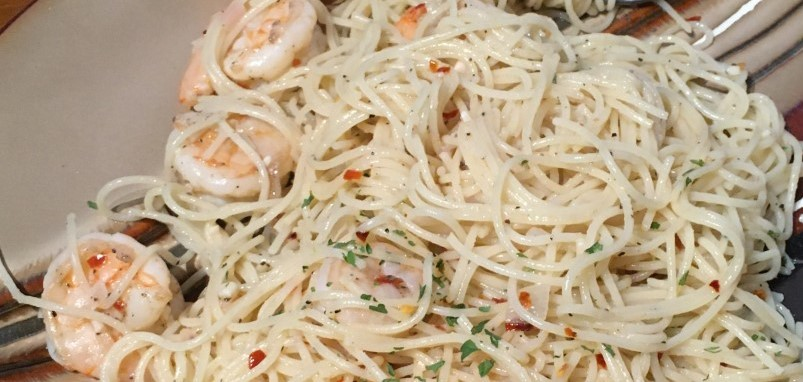
\includegraphics[scale=0.65]{Pasta/Shrimp Scampi/Shrimp Scampi.jpg}
%\end{center}


\end{document}